\chapter{Acides aminés et protéines}\label{ch:b1:proteins}

Faites cuire un œuf~: le blanc limpide devient opaque et ferme~; rien
n'a été ajouté ni retiré, mais chaque molécule de \omterm{def:b1:proteins:peptide}{protéine} s'y est
dépliée et emmêlée à ses voisines. Refroidissez-le~: il reste cuit. Et
pourtant une petite enzyme dépliée avec ménagement dans un tube à essai,
puis laissée dans un simple \omterm{def:b1:water-small-molecules:buffer}{tampon}, se replie en quelques minutes dans
sa forme de travail exacte, sans aucune aide~: la forme était écrite
dans la chaîne. Les \omterm{def:b1:proteins:peptide}{protéines} sont les molécules ouvrières de la \omterm{def:b1:cell-unit-of-life:cell}{cellule}
--- ses enzymes, ses \omterm{def:b1:membranes-transport:transporters}{pompes}, ses moteurs, ses charpentes, ses anticorps,
ses hormones --- et chacune est une chaîne d'\omterm{def:b1:proteins:aminoacid}{acides aminés} repliée dans
une forme que sa séquence dicte. Ce chapitre décrit les vingt \omterm{def:b1:proteins:aminoacid}{acides
aminés}, la liaison qui les unit, les quatre niveaux de structure des
\omterm{def:b1:proteins:peptide}{protéines}, le repliement qui fait d'une chaîne une machine, le
comportement coopératif des \omterm{def:b1:proteins:peptide}{protéines} à plusieurs sous-unités, et les
méthodes par lesquelles les \omterm{def:b1:proteins:peptide}{protéines} sont séparées et observées.

\section{Les acides aminés}

\begin{definition}[Acide aminé]\label{def:b1:proteins:aminoacid}
Un \emph{acide aminé}\index{acide amine@acide aminé} possède un \emph{carbone
$\alpha$} central portant un groupe aminé ($-\mathrm{NH_2}$), un groupe
carboxyle ($-\mathrm{COOH}$), un hydrogène et une \emph{chaîne
latérale}\index{chaine laterale@chaîne latérale} $R$ qui distingue les vingt acides
aminés standard des \omterm{def:b1:proteins:peptide}{protéines}. Au pH de la \omterm{def:b1:cell-unit-of-life:cell}{cellule}, le groupe aminé est
protoné et le carboxyle ionisé~: la molécule est un
\emph{zwitterion}\index{zwitterion},
$\mathrm{^+H_3N{-}CHR{-}COO^-}$, sans charge nette. Le carbone $\alpha$
est chiral chez tous sauf la glycine, et les êtres vivants n'emploient
que l'énantiomère L. Les chaînes latérales se groupent par leur
chimie~:
\begin{center}
\scriptsize
\begin{tabular}{lll}
\hline
classe & acides aminés (codes à trois et à une lettre) & chaîne latérale \\
\hline
apolaire, aliphatique & Gly G, Ala A, Val V, Leu L, Ile I, Met M, Pro P & hydrocarbonée~; Pro un cycle \\
aromatique & Phe F, Tyr Y, Trp W & cycles~; Tyr et Trp absorbent l'UV \\
\omterm{def:b1:water-small-molecules:water}{polaire}, non chargée & Ser S, Thr T, Cys C, Asn N, Gln Q & $-$OH, $-$SH, amide \\
chargée positivement & Lys K, Arg R, His H & bases~; His p$K_a$ 6.0 \\
chargée négativement & Asp D, Glu E & carboxylates, p$K_a$ 4 \\
\hline
\end{tabular}
\end{center}
Neuf d'entre eux (His, Ile, Leu, Lys, Met, Phe, Thr, Trp, Val) sont
\emph{indispensables} à l'humain~: nous ne savons pas les fabriquer et
devons les manger.
\end{definition}

\begin{proposition}[Ionisation]\label{prop:b1:proteins:ionisation}
Chaque groupe ionisable d'un \omterm{def:b1:proteins:aminoacid}{acide aminé} a son propre p$K_a$~: environ 2
pour le carboxyle $\alpha$, 9.5 pour l'aminé $\alpha$, et pour les
\omterm{def:b1:proteins:aminoacid}{chaînes latérales} 3.9 (Asp), 4.1 (Glu), 6.0 (His), 8.3 (Cys), 10.1
(Tyr), 10.5 (Lys), 12.5 (Arg). Le \emph{point
isoélectrique}\index{point isoelectrique@point isoélectrique} p$I$ est le pH auquel la
charge nette est nulle --- la moyenne des deux p$K_a$ qui encadrent la
forme neutre~; le p$I$ d'une \omterm{def:b1:proteins:peptide}{protéine} est fixé par sa teneur en \omterm{def:b1:proteins:aminoacid}{chaînes
latérales} chargées, et à ce pH elle est la moins soluble et ne migre pas
dans un champ électrique. L'histidine, dont le p$K_a$ est proche de 7,
est le résidu qui change de charge dans le domaine physiologique, et
elle siège dans le site actif de nombreuses enzymes.
\end{proposition}

\begin{omfigure}
\begin{tikzpicture}
\begin{axis}[
  width=0.86\linewidth, height=6.0cm,
  axis x line=bottom, axis y line=left,
  xmin=0, xmax=2.1, ymin=0, ymax=13,
  xlabel={équivalents de $\mathrm{OH^-}$ ajoutés}, ylabel={pH},
  xlabel style={font=\small, at={(axis description cs:0.5,-0.12)}, anchor=north},
  ylabel style={font=\small},
  tick label style={font=\small}, xtick={0,0.5,1,1.5,2}, ytick={0,2,4,6,8,10,12},
  clip=false,
]
\addplot[very thick, omDef, domain=0.02:0.98, samples=80] {2.34 + log10(x/(1-x))};
\addplot[very thick, omDef, domain=1.02:1.98, samples=80] {9.6 + log10((x-1)/(2-x))};
\addplot[very thick, omDef, domain=0.98:1.02, samples=10] {5.97 + (x-1)*250};
\draw[dashed, gray] (axis cs:0,2.34) -- (axis cs:0.5,2.34); \node[font=\scriptsize, anchor=west] at (axis cs:0.02,3.4) {p$K_1 = 2.34$~: $\mathrm{COOH}/\mathrm{COO^-}$};
\draw[dashed, gray] (axis cs:0,9.6) -- (axis cs:1.5,9.6); \node[font=\scriptsize, anchor=north west] at (axis cs:1.52,9.3) {p$K_2 = 9.6$~: $\mathrm{NH_3^+}/\mathrm{NH_2}$};
\draw[dashed, gray] (axis cs:0,5.97) -- (axis cs:1,5.97); \node[font=\scriptsize, anchor=south east] at (axis cs:0.98,6.1) {p$I = 5.97$~: zwitterion};
\node[font=\scriptsize, anchor=west] at (axis cs:0.42,0.9) {$\mathrm{^+H_3N{-}CH_2{-}COOH}$};
\node[font=\scriptsize, anchor=east] at (axis cs:0.93,8.5) {$\mathrm{^+H_3N{-}CH_2{-}COO^-}$};
\node[font=\scriptsize, anchor=south] at (axis cs:1.75,12.0) {$\mathrm{H_2N{-}CH_2{-}COO^-}$};
\end{axis}
\end{tikzpicture}

{\small Titrage de la glycine. Deux plateaux \omterm{def:b1:water-small-molecules:buffer}{tampons}, aux p$K_a$ du
carboxyle et du groupe aminé~; entre eux, au \omterm{prop:b1:proteins:ionisation}{point isoélectrique}, le
\omterm{def:b1:proteins:aminoacid}{zwitterion} ne porte aucune charge nette.}
\end{omfigure}

\section{La liaison peptidique}

\begin{definition}[Liaison peptidique, polypeptide]\label{def:b1:proteins:peptide}
La \emph{liaison peptidique}\index{liaison peptidique} unit le carboxyle
d'un \omterm{def:b1:proteins:aminoacid}{acide aminé} au groupe aminé du suivant par condensation (une
liaison amide, $\mathrm{-CO{-}NH-}$). Une chaîne d'\omterm{def:b1:proteins:aminoacid}{acides aminés} ainsi
unis est un \emph{polypeptide}\index{polypeptide}~: un \emph{squelette}
d'unités $\mathrm{N{-}C_\alpha{-}C}$ répétées d'où les \omterm{def:b1:proteins:aminoacid}{chaînes latérales}
font saillie, avec une \emph{extrémité N-terminale} (groupe aminé libre)
et une \emph{extrémité C-terminale} (carboxyle libre). Les séquences
s'écrivent de N vers C, l'ordre de la synthèse
(\cref{ch:b1:gene-expression}). Une \emph{protéine}\index{proteine@protéine} est
un ou plusieurs polypeptides repliés en une forme définie~; les chaînes
usuelles comptent \qtyrange{100}{1000}{} résidus de masse moyenne
\qty{110}{Da}, de sorte qu'une protéine de \qty{300}{} résidus fait
\qty{33}{kDa}.
\end{definition}

\begin{proposition}[Géométrie de la liaison peptidique]\label{prop:b1:proteins:geometry}
La liaison C--N d'un peptide a un caractère partiel de double liaison
(la résonance de l'amide)~: elle est courte, ne peut pas tourner, et
maintient les six atomes
$\mathrm{C_\alpha{-}C(=O){-}N(H){-}C_\alpha}$ dans un même plan, presque
toujours avec les deux carbones $\alpha$ en \emph{trans}. Le squelette
est donc une chaîne de plans rigides articulés aux carbones $\alpha$,
chaque articulation ayant deux rotations, $\phi$ (autour de
N--$\mathrm{C_\alpha}$) et $\psi$ (autour de $\mathrm{C_\alpha}$--C), et
les gênes stériques entre \omterm{def:b1:proteins:aminoacid}{chaînes latérales} et squelette interdisent la
plupart des combinaisons de $\phi$ et de $\psi$. La conformation d'une
\omterm{def:b1:proteins:peptide}{protéine} est essentiellement la liste de ses angles $\phi$ et $\psi$.
\end{proposition}

\begin{omfigure}
\begin{tikzpicture}[font=\footnotesize, line cap=round]
  % two peptide planes
  \fill[omDef!12, rounded corners=3pt] (0.3,-0.9) rectangle (3.3,0.9);
  \fill[omDef!12, rounded corners=3pt] (3.9,-0.9) rectangle (6.9,0.9);
  % atoms
  \node (ca1) at (0,0) {$\mathrm{C_\alpha}$};
  \node (c1) at (1.2,0.4) {C};
  \node (o1) at (1.2,1.3) {O};
  \node (n1) at (2.4,-0.4) {N};
  \node (h1) at (2.4,-1.3) {H};
  \node (ca2) at (3.6,0) {$\mathrm{C_\alpha}$};
  \node (c2) at (4.8,0.4) {C};
  \node (o2) at (4.8,1.3) {O};
  \node (n2) at (6.0,-0.4) {N};
  \node (h2) at (6.0,-1.3) {H};
  \node (ca3) at (7.2,0) {$\mathrm{C_\alpha}$};
  \draw[thick] (ca1) -- (c1); \draw[thick, double] (c1) -- (o1); \draw[very thick, omThm] (c1) -- (n1); \draw[thick] (n1) -- (h1); \draw[thick] (n1) -- (ca2);
  \draw[thick] (ca2) -- (c2); \draw[thick, double] (c2) -- (o2); \draw[very thick, omThm] (c2) -- (n2); \draw[thick] (n2) -- (h2); \draw[thick] (n2) -- (ca3);
  % side chains
  \draw[thick] (ca1) -- ++(-0.5,-0.8) node[below] {$R_1$};
  \draw[thick] (ca2) -- ++(0,-1.0) node[below] {$R_2$};
  \draw[thick] (ca3) -- ++(0.5,-0.8) node[below] {$R_3$};
  % rotation arrows phi/psi at ca2
  \draw[->, omProp, thick] (2.9,-0.55) arc (200:340:0.35); \node[omProp, font=\scriptsize] at (3.05,-0.95) {$\phi$};
  \draw[->, omProp, thick] (3.85,0.55) arc (160:20:0.35); \node[omProp, font=\scriptsize] at (4.2,1.0) {$\psi$};
  \node[anchor=west, align=left] at (7.9,0.6) {\textcolor{omThm}{rouge}~: la liaison peptidique, plane,\\ sans rotation (double liaison partielle)};
  \node[anchor=west, align=left] at (7.9,-0.5) {\textcolor{omProp}{orange}~: les deux rotations libres\\ $\phi$ et $\psi$ à chaque carbone $\alpha$};
\end{tikzpicture}

{\small Deux \omterm{def:b1:proteins:peptide}{liaisons peptidiques}. Chaque plan grisé tient six atomes
rigidement~; la chaîne ne fléchit qu'aux carbones $\alpha$, par les
angles $\phi$ et $\psi$.}
\end{omfigure}

\section{La structure secondaire}

\begin{definition}[Structure secondaire]\label{def:b1:proteins:secondary}
La \emph{structure secondaire}\index{structure secondaire} d'une
\omterm{def:b1:proteins:peptide}{protéine} est le repliement local et régulier de son squelette, tenu par
des \omterm{def:b1:water-small-molecules:water}{liaisons hydrogène} entre les groupes C=O et N--H du squelette. Deux
motifs dominent. L'\emph{hélice $\alpha$}\index{helice alpha@hélice $\alpha$}~:
une spirale droite de 3.6 résidus par tour, s'élevant de \qty{0.15}{nm}
par résidu (\qty{0.54}{nm} par tour), chaque C=O étant lié au N--H situé
quatre résidus plus loin, les \omterm{def:b1:proteins:aminoacid}{chaînes latérales} pointant vers
l'extérieur. Le \emph{feuillet
$\beta$}\index{feuillet beta@feuillet $\beta$}~: des chaînes presque
entièrement étirées (\qty{0.35}{nm} par résidu) et disposées côte à
côte, parallèles ou antiparallèles, liées entre brins voisins, les
\omterm{def:b1:proteins:aminoacid}{chaînes latérales} alternant au-dessus et au-dessous du feuillet. Entre
eux, des \emph{coudes} et des boucles inversent le sens de la chaîne. La
proline, dont le cycle bloque $\phi$, brise les hélices~; la glycine,
sans \omterm{def:b1:proteins:aminoacid}{chaîne latérale}, permet des coudes qu'aucun autre résidu ne peut
faire.
\end{definition}

\begin{omfigure}
\begin{tikzpicture}
\begin{axis}[
  width=0.62\linewidth, height=6.4cm,
  axis x line=bottom, axis y line=left,
  xmin=-180, xmax=180, ymin=-180, ymax=180,
  xlabel={$\phi$ (degrés)}, ylabel={$\psi$ (degrés)},
  xlabel style={font=\small, at={(axis description cs:0.5,-0.12)}, anchor=north},
  ylabel style={font=\small},
  tick label style={font=\small}, xtick={-180,-90,0,90,180}, ytick={-180,-90,0,90,180},
  clip=false,
]
\fill[omDef!35] (axis cs:-160,90) rectangle (axis cs:-50,180);
\fill[omDef!35] (axis cs:-160,-180) rectangle (axis cs:-50,-150);
\fill[omThm!35] (axis cs:-150,-70) rectangle (axis cs:-45,-10);
\fill[omExo!35] (axis cs:40,10) rectangle (axis cs:80,70);
\node[font=\scriptsize] at (axis cs:-105,140) {feuillet $\beta$};
\node[font=\scriptsize] at (axis cs:-97,-40) {hélice $\alpha$ droite};
\node[font=\scriptsize, align=center] at (axis cs:60,100) {hélice gauche\\ (glycine seule)};
\node[font=\scriptsize, gray, align=center] at (axis cs:80,-100) {blanc~: interdit par\\ les gênes stériques};
\draw[gray] (axis cs:-180,0) -- (axis cs:180,0); \draw[gray] (axis cs:0,-180) -- (axis cs:0,180);
\end{axis}
\end{tikzpicture}

{\small Le diagramme de Ramachandran~: les combinaisons de $\phi$ et de
$\psi$ qu'un résidu peut adopter. Deux grandes régions autorisées
correspondent au feuillet $\beta$ et à l'hélice $\alpha$ droite~; la
plus grande partie du plan est interdite par les collisions entre
atomes.}
\end{omfigure}

\begin{omfigure}
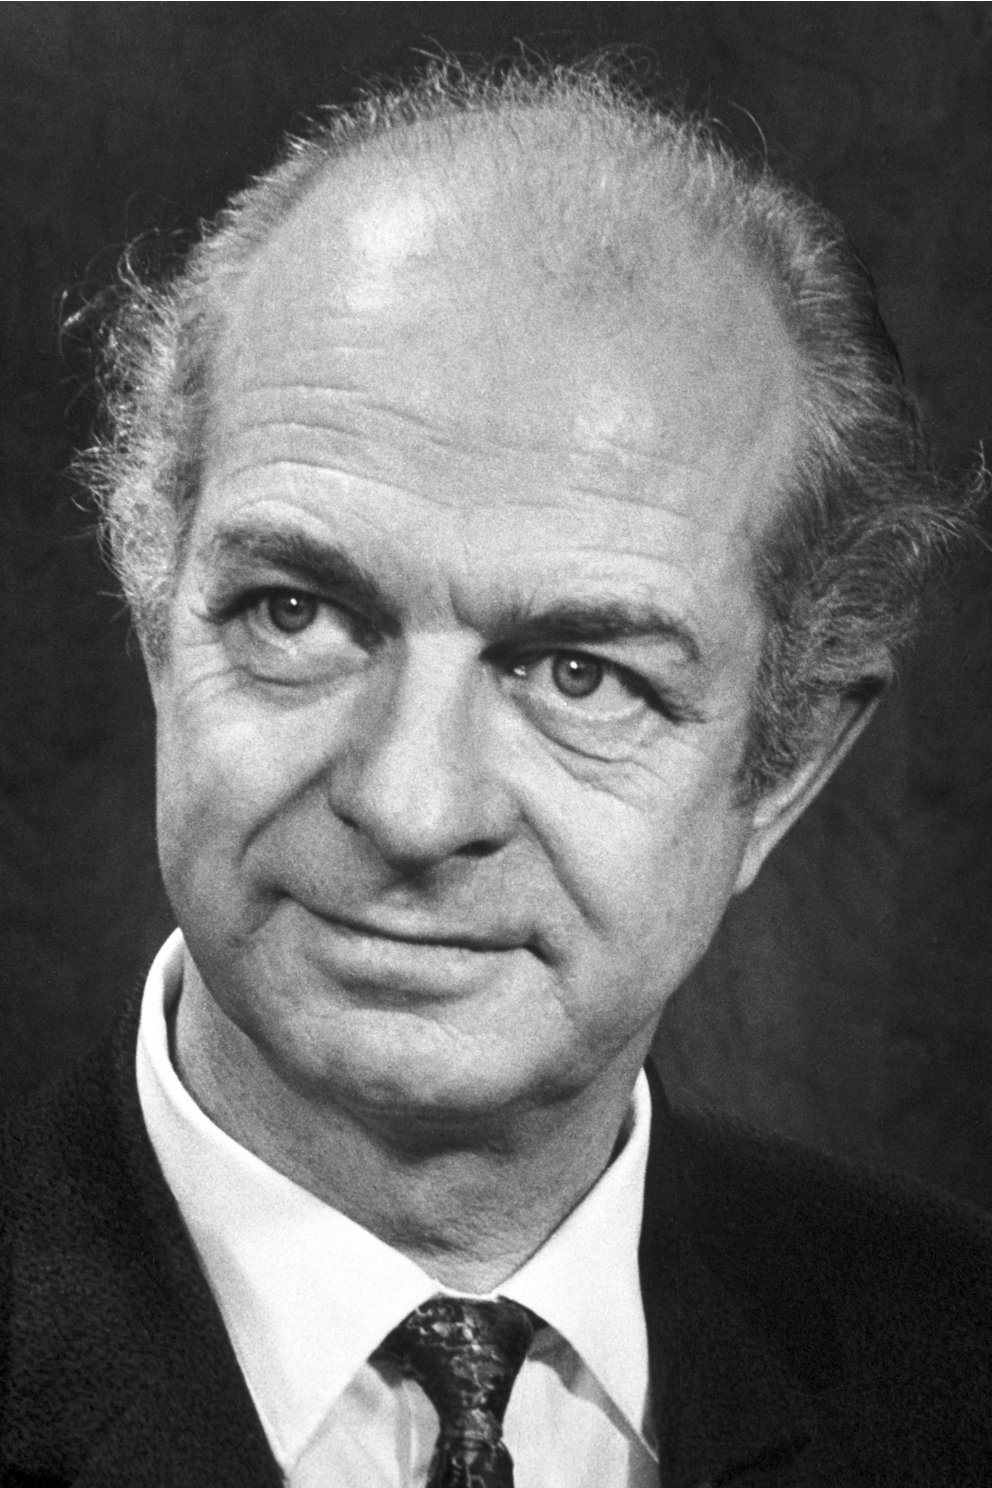
\includegraphics[width=0.26\linewidth]{images/book3/pauling.jpg}

{\small Linus Pauling (1901--1994), qui déduisit l'hélice $\alpha$ et le
feuillet $\beta$ en 1951 de la planéité de la \omterm{def:b1:proteins:peptide}{liaison peptidique} et de
la géométrie des \omterm{def:b1:water-small-molecules:water}{liaisons hydrogène}, avant que l'une ou l'autre n'ait
été vue dans une \omterm{def:b1:proteins:peptide}{protéine}. Photographie~: Fondation Nobel, 1962,
domaine public.}
\end{omfigure}

\begin{example}[Hélice et feuillet en chiffres]\label{ex:b1:proteins:numbers}
Une hélice $\alpha$ qui traverse une membrane doit franchir \qty{3}{nm}
de cœur hydrophobe~: $3/0.15 = 20$ résidus, et de fait les segments
transmembranaires du \cref{ch:b1:membranes-transport} sont des suites
d'une vingtaine de résidus hydrophobes. Un brin $\beta$ de même longueur
couvre \qty{7}{nm}~: la fibroïne de la soie est faite de feuillets
antiparallèles empilés de glycine et d'alanine, et un fil de soie est
plus résistant que de l'acier de même masse parce que les squelettes
covalents s'alignent le long de la fibre.
\end{example}

\section{Structures tertiaire et quaternaire}

\begin{definition}[Structures tertiaire et quaternaire]\label{def:b1:proteins:tertiary}
La \emph{structure tertiaire}\index{structure tertiaire} est
l'arrangement tridimensionnel complet d'un \omterm{def:b1:proteins:peptide}{polypeptide}~: ses hélices,
ses feuillets et ses boucles tassés ensemble, souvent en plusieurs
\emph{domaines} compacts qui se replient indépendamment. Elle est tenue
par des forces non covalentes --- l'\emph{\omterm{prop:b1:water-small-molecules:properties}{effet hydrophobe}} qui enfouit
les \omterm{def:b1:proteins:aminoacid}{chaînes latérales} apolaires dans un cœur à l'abri de l'eau, des
\omterm{def:b1:water-small-molecules:water}{liaisons hydrogène}, des ponts salins entre \omterm{def:b1:proteins:aminoacid}{chaînes latérales} chargées,
un tassement de \omterm{def:b1:water-small-molecules:bonds}{van der Waals} --- et parfois par des \emph{ponts
disulfure}\index{pont disulfure}, \omterm{def:b1:water-small-molecules:bonds}{liaisons covalentes} S--S entre deux
cystéines, dans les \omterm{def:b1:proteins:peptide}{protéines} sécrétées vers l'extérieur oxydant. La
\emph{structure quaternaire}\index{structure quaternaire} est
l'assemblage de plusieurs \omterm{def:b1:proteins:peptide}{polypeptides} (sous-unités) en une seule
\omterm{def:b1:proteins:peptide}{protéine}~: l'hémoglobine est faite de deux chaînes $\alpha$ et de deux
chaînes $\beta$. Les \omterm{def:b1:proteins:peptide}{protéines} \emph{globulaires} sont compactes et
hydrosolubles (enzymes, transporteurs)~; les \omterm{def:b1:proteins:peptide}{protéines}
\emph{fibreuses} sont étirées et insolubles (triple hélice du
\omterm{def:b1:body-plans-tissues:connective}{collagène}, hélices superenroulées de la kératine et de la myosine,
soie).
\end{definition}

\begin{omfigure}
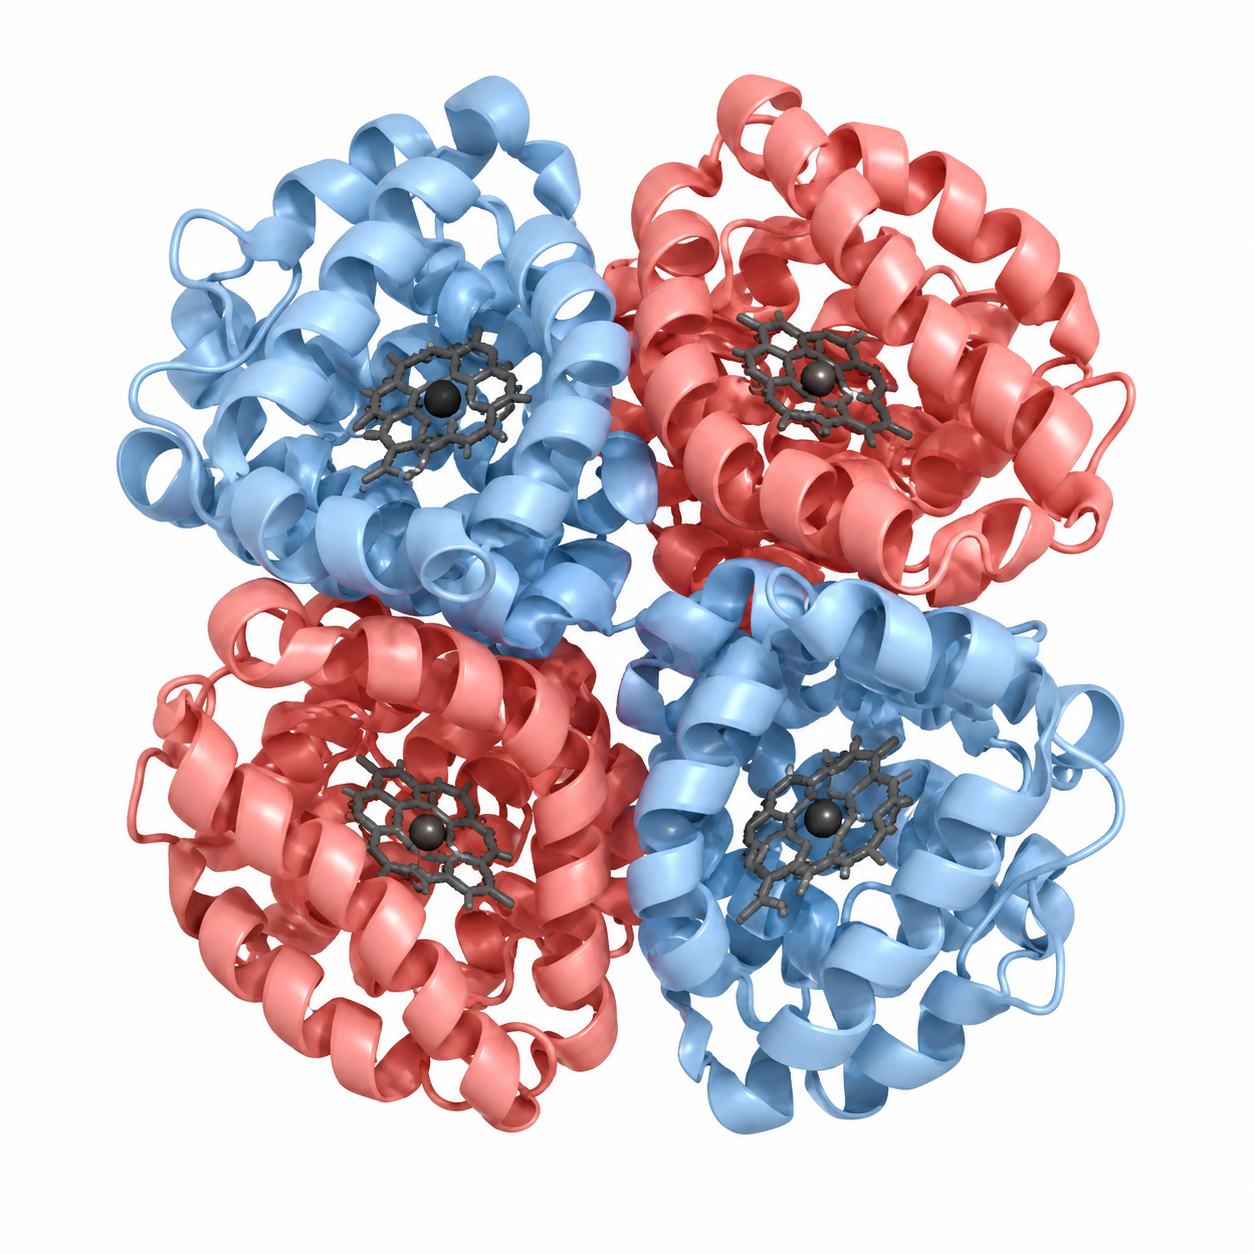
\includegraphics[width=0.42\linewidth]{images/book3/ai/fig-hemoglobin-ribbon.png}

{\small L'hémoglobine~: quatre sous-unités, deux $\alpha$ (bleu) et deux
$\beta$ (rouge), chacune formant un faisceau d'hélices $\alpha$ autour
d'un groupe hème (sombre) dont le fer fixe un $\mathrm{O_2}$. Les quatre
sites n'agissent pas indépendamment.}
\end{omfigure}

\begin{theorem}[La séquence détermine le repliement]\label{thm:b1:proteins:anfinsen}
\index{repliement des proteines@repliement des protéines}
La structure tridimensionnelle d'une \omterm{def:b1:proteins:peptide}{protéine} est déterminée par sa
séquence d'\omterm{def:b1:proteins:aminoacid}{acides aminés}~: le repliement natif est la conformation
d'\omterm{prop:b1:water-small-molecules:gibbs}{énergie libre} la plus basse que la chaîne puisse atteindre dans son
environnement cellulaire, et l'information nécessaire pour l'atteindre
est contenue dans la chaîne elle-même.
\end{theorem}
\begin{proof}[Faits expérimentaux]
Anfinsen (1961) déplia la ribonucléase A, enzyme de \qty{124}{} résidus
à quatre \omterm{def:b1:proteins:tertiary}{ponts disulfure}, dans de l'urée concentrée avec un réducteur
qui rompait les ponts~: la chaîne perdit toute activité. En retirant
l'urée et en laissant les cystéines se réoxyder lentement à l'air, il
récupéra l'enzyme pleinement active, ses quatre ponts reformés entre les
huit mêmes cystéines parmi les \qty{105}{} appariements possibles ---
la chaîne avait trouvé son propre repliement. Réoxydée alors qu'elle
était encore dans l'urée, elle formait des ponts au hasard et restait
inactive~; une trace de réducteur lui permettait ensuite de les
rebrasser jusqu'à atteindre le jeu natif, le plus stable. Depuis, des
milliers de séquences ont été repliées à partir de rien dans le tube à
essai, et le repliement d'une séquence nouvelle peut désormais en être
calculé.
\end{proof}

\begin{proposition}[Dénaturation]\label{prop:b1:proteins:denaturation}
\index{denaturation (proteine)@dénaturation (protéine)}
La chaleur, les pH extrêmes, l'urée, les détergents ou les solvants
organiques déplient les \omterm{def:b1:proteins:peptide}{protéines} en submergeant les liaisons faibles
qui tiennent le repliement~: la chaîne perd sa forme et sa fonction,
expose son cœur hydrophobe et s'agrège avec ses voisines. Les petites
\omterm{def:b1:proteins:peptide}{protéines} se replient de nouveau quand on retire le dénaturant~; les
grandes, et les \omterm{def:b1:proteins:peptide}{protéines} d'une \omterm{def:b1:cell-unit-of-life:cell}{cellule} encombrée, souvent non, et la
\omterm{def:b1:cell-unit-of-life:cell}{cellule} entretient des \emph{chaperons}\index{chaperon} --- \omterm{def:b1:proteins:peptide}{protéines}
qui lient les chaînes dépliées, masquent leurs surfaces hydrophobes et
leur offrent des chances répétées de se replier correctement --- et
détruit ce qui reste mal replié. Une fièvre de quelques degrés, et les
\qty{42}{\celsius} auxquels les \omterm{def:b1:proteins:peptide}{protéines} de l'encéphale commencent à se
déplier, marquent l'étroite marge de stabilité~: un repliement typique
n'est que de \qtyrange{20}{60}{kJ/mol} plus stable que la chaîne
dépliée, la valeur de quelques \omterm{def:b1:water-small-molecules:water}{liaisons hydrogène}.
\end{proposition}

\begin{omfigure}
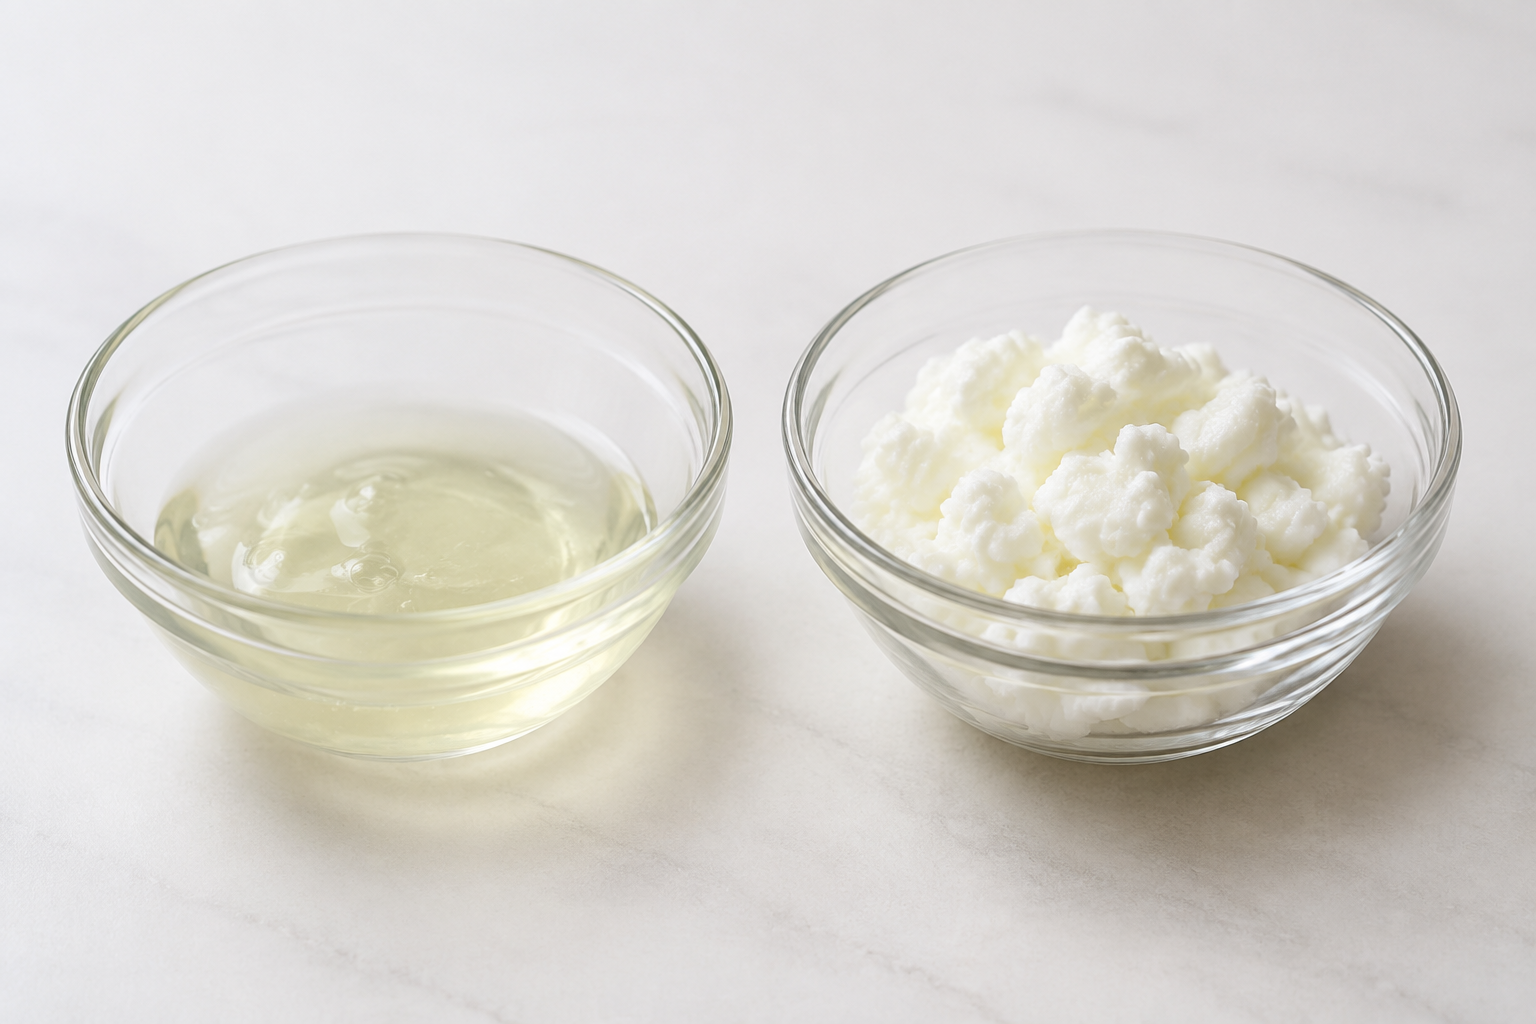
\includegraphics[width=0.5\linewidth]{images/book3/ai/b3-12-egg-white-cooked.png}

{\small Blanc d'œuf cru et cuit~: les mêmes \omterm{def:b1:proteins:peptide}{protéines}, repliées et
solubles à gauche, dépliées et agrégées en un solide opaque à droite.
Rien n'a été ajouté que de la chaleur.}
\end{omfigure}

\begin{example}[Le collagène]\label{ex:b1:proteins:collagen}
Le quart des \omterm{def:b1:proteins:peptide}{protéines} d'un mammifère est du \omterm{def:b1:body-plans-tissues:connective}{collagène}~: trois chaînes,
chacune une hélice gauche de mille résidus avec une glycine une position
sur trois (Gly--X--Y, Y souvent une hydroxyproline), enroulées ensemble
en une triple hélice droite longue de \qty{300}{nm}, puis empaquetées
côte à côte en fibrilles réticulées par des \omterm{def:b1:water-small-molecules:bonds}{liaisons covalentes}.
L'absence de \omterm{def:b1:proteins:aminoacid}{chaîne latérale} chez la glycine est ce qui permet aux trois
chaînes de se tasser sur l'axe~; une seule substitution de glycine par
un autre résidu coude l'hélice et donne des os cassants. La vitamine C
est nécessaire pour hydroxyler les prolines~; sans elle l'hélice est
instable et les fibrilles cèdent~: c'est le scorbut.
\end{example}

\section{L'allostérie~: l'hémoglobine}

\begin{definition}[Allostérie, coopérativité]\label{def:b1:proteins:allostery}
Une \omterm{def:b1:proteins:peptide}{protéine} est \emph{allostérique}\index{allosterie@allostérie} lorsque la
fixation d'un ligand sur un site change la conformation de la \omterm{def:b1:proteins:peptide}{protéine}
et, par là, son affinité en un autre site. Lorsque les sites sont
semblables et que le changement augmente l'affinité des autres, la
fixation est \emph{coopérative}\index{cooperativite@coopérativité}~: la courbe de
saturation est sigmoïde plutôt qu'hyperbolique, et la \omterm{def:b1:proteins:peptide}{protéine} bascule
de presque vide à presque pleine sur un étroit domaine de concentration
du ligand. L'\emph{équation de Hill}\index{equation de Hill@équation de Hill} la décrit~:
\[
Y = \frac{P^n}{P_{50}^n + P^n},
\]
où $Y$ est la fraction des sites occupés, $P$ la concentration du ligand
(ou sa pression partielle), $P_{50}$ la valeur à la demi-saturation, et
$n$ le coefficient de Hill --- 1 pour des sites indépendants, jusqu'au
nombre de sites pour une coopérativité parfaite.
\end{definition}

\begin{proposition}[Hémoglobine et myoglobine]\label{prop:b1:proteins:hemoglobin}
La myoglobine, une chaîne à un seul hème, fixe l'$\mathrm{O_2}$ selon
une hyperbole ($n = 1$, $P_{50} = \qty{0.37}{kPa}$)~: elle est saturée à
toute pression que les \omterm{def:b1:body-plans-tissues:tissue}{tissus} offrent et sert de réserve dans le muscle.
L'hémoglobine, quatre sous-unités, fixe de façon \omterm{def:b1:proteins:allostery}{coopérative}
($n \approx 2.8$, $P_{50} = \qty{3.5}{kPa}$)~: le premier
$\mathrm{O_2}$ fixé fait basculer le tétramère d'un \emph{état T} de
faible affinité vers un \emph{état R} de forte affinité, de sorte
qu'elle se charge presque complètement aux \qty{13}{kPa} du poumon et
décharge une large fraction aux \qty{5}{kPa} des \omterm{def:b1:body-plans-tissues:tissue}{tissus}. Son affinité
est encore abaissée, et la décharge favorisée, par l'acidité et le
$\mathrm{CO_2}$ (l'\emph{effet Bohr}) et par le
2,3-bisphosphoglycérate (BPG), qui se lie à l'état T~: dans un muscle
qui travaille, ou en altitude, davantage d'oxygène est libéré à pression
égale. Le fœtus fabrique une hémoglobine qui lie faiblement le BPG, de
sorte que son sang tire l'oxygène de celui de la mère à travers le
placenta.
\end{proposition}

\begin{omfigure}
\begin{tikzpicture}
\begin{axis}[
  width=0.9\linewidth, height=6.4cm,
  axis x line=bottom, axis y line=left,
  xmin=0, xmax=14, ymin=0, ymax=1.08,
  xlabel={pression partielle d'$\mathrm{O_2}$ (\unit{kPa})}, ylabel={fraction des sites occupés $Y$},
  xlabel style={font=\small, at={(axis description cs:0.5,-0.12)}, anchor=north},
  ylabel style={font=\small},
  tick label style={font=\small}, xtick={0,2,4,6,8,10,12,14}, ytick={0,0.25,0.5,0.75,1},
  legend style={font=\small, at={(0.97,0.35)}, anchor=north east, draw=none},
  clip=false,
]
\addplot[very thick, omDef, domain=0.01:14, samples=120] {x/(0.37+x)};
\addlegendentry{myoglobine, $n=1$, $P_{50} = \qty{0.37}{kPa}$}
\addplot[very thick, omThm, domain=0.01:14, samples=120] {x^2.8/(3.5^2.8+x^2.8)};
\addlegendentry{hémoglobine, $n=2.8$, $P_{50} = \qty{3.5}{kPa}$}
\addplot[very thick, omProp, dashed, domain=0.01:14, samples=120] {x^2.8/(4.5^2.8+x^2.8)};
\addlegendentry{hémoglobine en milieu acide, $P_{50} = \qty{4.5}{kPa}$ (Bohr)}
\draw[dashed, gray] (axis cs:13.3,0) -- (axis cs:13.3,1.0); \node[font=\scriptsize, anchor=south] at (axis cs:13.3,1.01) {poumons};
\draw[dashed, gray] (axis cs:5.3,0) -- (axis cs:5.3,0.76); \node[font=\scriptsize, anchor=west] at (axis cs:5.45,0.07) {tissus};
\end{axis}
\end{tikzpicture}

{\small Fixation de l'oxygène par la myoglobine (hyperbolique) et par
l'hémoglobine (sigmoïde). Entre les poumons et les \omterm{def:b1:body-plans-tissues:tissue}{tissus}, la
myoglobine ne libère presque rien~; l'hémoglobine libère le cinquième
de sa charge, et davantage quand le \omterm{def:b1:body-plans-tissues:tissue}{tissu} est acide.}
\end{omfigure}

\begin{method}[Utiliser l'équation de Hill]\label{met:b1:proteins:hill}
\begin{enumerate}
  \item Lire $P_{50}$ sur la courbe en $Y = 0.5$~; estimer $n$ par la
        pente de $\log[Y/(1-Y)]$ en fonction de $\log P$ (le
        diagramme de Hill), qui est une droite de pente $n$ au
        voisinage de $P_{50}$.
  \item Calculer $Y$ à la pression de charge (poumons) et à la pression
        de décharge (\omterm{def:b1:body-plans-tissues:tissue}{tissus})~; la différence est la fraction de la
        capacité de transport effectivement délivrée.
  \item Multiplier par la capacité~: le sang contient \qty{150}{g/L}
        d'hémoglobine, chaque gramme fixant \qty{1.34}{mL}
        d'$\mathrm{O_2}$, soit \qty{200}{mL} d'$\mathrm{O_2}$ par litre
        à saturation.
  \item Pour tenir compte de l'effet Bohr ou du BPG, employer le
        $P_{50}$ décalé aux \omterm{def:b1:body-plans-tissues:tissue}{tissus} seulement, là où se trouve l'acide.
\end{enumerate}
\end{method}

\section{Voir et séparer les protéines}

\begin{method}[Séparer les protéines]\label{met:b1:proteins:methods}
\begin{enumerate}
  \item \emph{Électrophorèse en SDS}~: le détergent enrobe chaque chaîne
        d'une charge négative proportionnelle à sa longueur, de sorte
        que les chaînes migrent dans un gel de polyacrylamide selon leur
        seule taille~; une échelle de masses connues étalonne le gel, et
        la position d'une bande colorée donne la masse à quelques pour
        cent près.
  \item \emph{Chromatographie}~: à travers une colonne de billes qui
        retardent les \omterm{def:b1:proteins:peptide}{protéines} selon la taille (filtration sur gel~:
        les grandes sortent les premières), selon la charge (échange
        d'ions), ou par une liaison spécifique (affinité~: un ligand
        immobilisé retient une \omterm{def:b1:proteins:peptide}{protéine} et laisse passer le reste). Une
        purification se suit par la montée de l'activité spécifique
        (\cref{ch:b1:cell-unit-of-life}).
  \item \emph{Séquençage}~: la séquence du gène, traduite~; ou la
        \omterm{def:b1:proteins:peptide}{protéine} elle-même, coupée en peptides et lue par spectrométrie
        de masse.
  \item \emph{Structure}~: la diffraction des rayons X d'un cristal, ou
        la microscopie électronique de particules isolées congelées,
        donne la position de chaque atome~; les rubans dessinés dans ce
        chapitre en sont les résumés.
\end{enumerate}
\end{method}

\begin{omfigure}
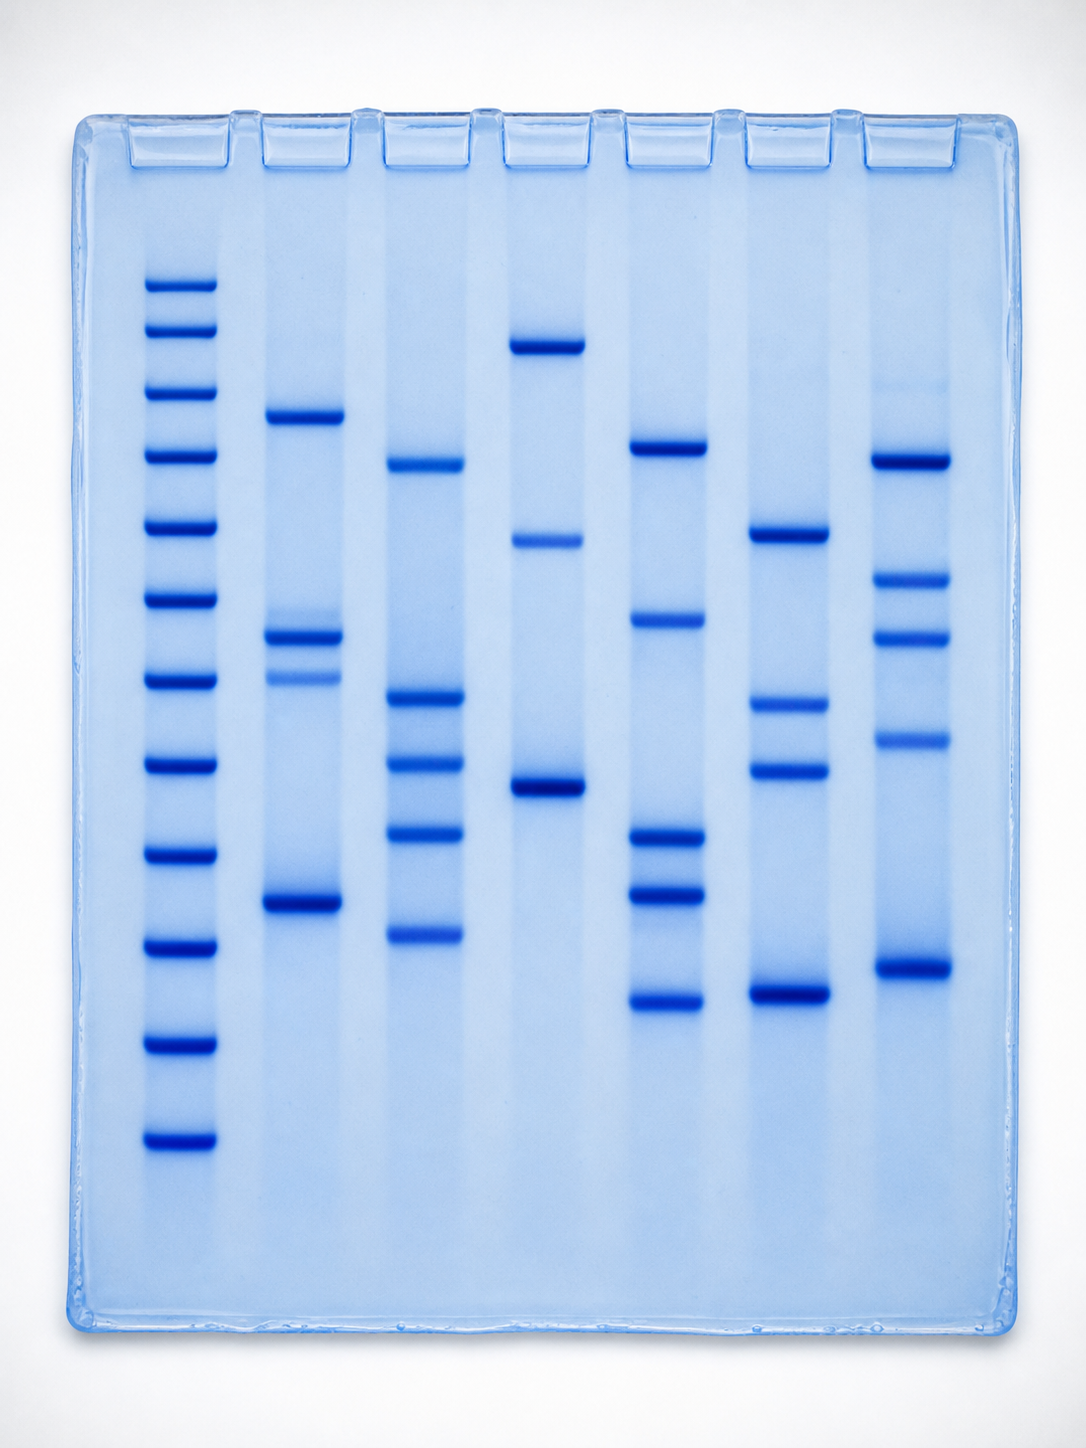
\includegraphics[width=0.36\linewidth]{images/book3/ai/b3-12-protein-gel.png}

{\small Un gel de polyacrylamide--SDS coloré. Chaque piste est un
échantillon~; chaque bande une \omterm{def:b1:proteins:peptide}{protéine} d'une taille~; la piste de
gauche une échelle de marqueurs de masse connue. Les petites \omterm{def:b1:proteins:peptide}{protéines}
migrent plus loin.}
\end{omfigure}

\begin{example}[Lire un gel]\label{ex:b1:proteins:gel}
Un extrait brut montre des dizaines de bandes~; après chromatographie
d'affinité, il reste une bande à la position du marqueur de
\qty{33}{kDa}. Migrée sans SDS et sans réducteur, la même \omterm{def:b1:proteins:peptide}{protéine} se
déplace comme une espèce de \qty{66}{kDa}~: c'est un dimère de deux
chaînes identiques tenues par un \omterm{def:b1:proteins:tertiary}{pont disulfure}, que le réducteur rompt
et que le détergent sépare. Deux gels, un seul raisonnement, et la
\omterm{def:b1:proteins:tertiary}{structure quaternaire} est connue.
\end{example}

\section{Exercices}

\begin{exercise}[$\star$]\label{exo:b1:proteins:1}
Dessiner ou décrire la structure générale d'un \omterm{def:b1:proteins:aminoacid}{acide aminé} à pH 7, et
classer Leu, Ser, Lys, Glu et Phe par \omterm{def:b1:proteins:aminoacid}{chaîne latérale}.
\end{exercise}

\begin{exercise}[$\star$]\label{exo:b1:proteins:2}
Définir les quatre niveaux de structure d'une \omterm{def:b1:proteins:peptide}{protéine} et les liaisons
qui tiennent chacun.
\end{exercise}

\begin{exercise}[$\star$]\label{exo:b1:proteins:3}
Une \omterm{def:b1:proteins:peptide}{protéine} compte \qty{450}{} résidus. Estimer sa masse. Si elle était
une hélice $\alpha$ unique, quelle serait sa longueur~? Et un brin
$\beta$ unique~?
\end{exercise}

\begin{exercise}[$\star$]\label{exo:b1:proteins:4}
D'après la figure de la fixation de l'oxygène, lire la saturation de
l'hémoglobine à \qty{13.3}{kPa} et à \qty{5.3}{kPa}, et la fraction
délivrée.
\end{exercise}

\begin{exercise}[$\star\star$]\label{exo:b1:proteins:5}
Calculer la charge nette du peptide Lys--Gly--Asp--Ala à pH 7, à pH 2 et
à pH 12, à l'aide des p$K_a$ du chapitre, et estimer son \omterm{prop:b1:proteins:ionisation}{point
isoélectrique}.
\end{exercise}

\begin{exercise}[$\star\star$]\label{exo:b1:proteins:6}
Expliquer pourquoi la proline se rencontre rarement à l'intérieur des
hélices $\alpha$ et pourquoi la glycine se trouve aux coudes serrés, à
partir de la géométrie du squelette.
\end{exercise}

\begin{exercise}[$\star\star$]\label{exo:b1:proteins:7}
Dans l'expérience d'Anfinsen, quelle fraction des réoxydations
aléatoires donnerait le jeu natif de quatre \omterm{def:b1:proteins:tertiary}{ponts disulfure}~? (Compter
les manières d'apparier huit cystéines.) Qu'a prouvé la récupération
effective de la pleine activité~?
\end{exercise}

\begin{exercise}[$\star\star$]\label{exo:b1:proteins:8}
À l'aide de l'\omterm{def:b1:proteins:allostery}{équation de Hill} avec $n = 2.8$ et
$P_{50} = \qty{3.5}{kPa}$, calculer $Y$ à \qty{2}{kPa}, à
\qty{3.5}{kPa} et à \qty{8}{kPa}. Reprendre avec $n = 1$. Quelle
\omterm{def:b1:proteins:peptide}{protéine} délivre le plus entre \qty{8}{} et \qty{2}{kPa}~?
\end{exercise}

\begin{exercise}[$\star\star$]\label{exo:b1:proteins:9}
Une \omterm{def:b1:proteins:peptide}{protéine} migre en une seule bande de \qty{50}{kDa} sur un gel SDS et
sort d'une colonne de filtration sur gel à \qty{200}{kDa}. Donner sa
\omterm{def:b1:proteins:tertiary}{structure quaternaire} et dire comment on vérifierait la présence de
\omterm{def:b1:proteins:tertiary}{ponts disulfure} entre les sous-unités.
\end{exercise}

\begin{exercise}[$\star\star\star$]\label{exo:b1:proteins:10}
L'hémoglobine drépanocytaire porte une valine au lieu d'un glutamate en
position 6 de la chaîne $\beta$, à la surface. Expliquer, à partir de la
chimie des deux \omterm{def:b1:proteins:aminoacid}{chaînes latérales}, pourquoi la \omterm{def:b1:proteins:peptide}{protéine} mutée
polymérise lorsqu'elle est désoxygénée, et pourquoi la maladie se
manifeste dans les \omterm{def:b1:body-plans-tissues:tissue}{tissus} plutôt que dans les poumons.
\end{exercise}

\begin{exercise}[$\star\star\star$]\label{exo:b1:proteins:11}
Un repliement n'est stable que de \qty{40}{kJ/mol}. Calculer la fraction
de molécules dépliées à l'équilibre à \qty{37}{\celsius}
($K = e^{-\Delta G/RT}$), puis à \qty{45}{\celsius} si $\Delta G$ est
tombé à \qty{10}{kJ/mol}. Pourquoi une stabilité aussi marginale est-elle
utile à une \omterm{def:b1:cell-unit-of-life:cell}{cellule}~?
\end{exercise}

\begin{exercise}[$\star\star\star$]\label{exo:b1:proteins:12}
«~Une \omterm{def:b1:proteins:peptide}{protéine} est une séquence qui se replie en une forme, et la forme
est la fonction.~» Discuter en un paragraphe à l'aide d'Anfinsen, des
\omterm{prop:b1:proteins:denaturation}{chaperons}, de la drépanocytose et de l'\omterm{def:b1:proteins:allostery}{allostérie}~: où la phrase tient
et où la \omterm{def:b1:cell-unit-of-life:cell}{cellule} doit intervenir.
\end{exercise}

\section{Problème~: l'hémoglobine au travail}

\begin{problem}[{Problème du week-end --- l'oxygène porté du poumon au
muscle, au repos, en sprint, en montagne et avant la naissance, jusqu'à
l'oxygène délivré par litre de sang}]
\label{pb:b1:proteins:1}
Le sang contient \qty{150}{g/L} d'hémoglobine~; \qty{1}{g} fixe
\qty{1.34}{mL} d'$\mathrm{O_2}$. L'hémoglobine obéit à l'\omterm{def:b1:proteins:allostery}{équation de
Hill} avec $n = 2.8$ et $P_{50} = \qty{3.5}{kPa}$ à pH 7.4~; la
myoglobine a $n = 1$ et $P_{50} = \qty{0.37}{kPa}$. Pressions
partielles d'$\mathrm{O_2}$~: \qty{13.3}{kPa} dans les poumons au niveau
de la mer, \qty{5.3}{kPa} dans les \omterm{def:b1:body-plans-tissues:tissue}{tissus} au repos. Prendre
$2.8\ln 3.5 = 3.51$,
$2.8\ln 5.3 = 4.67$, $2.8\ln 13.3 = 7.25$, $2.8\ln 2.7 = 2.78$,
$2.8\ln 4.5 = 4.21$, $2.8\ln 7 = 5.45$, $2.8\ln 4 = 3.88$,
$2.8\ln 2.6 = 2.68$.

\medskip
\noindent\textbf{Partie I --- Au repos.}
\begin{enumerate}
  \item Calculer la capacité en oxygène d'un litre de sang.
  \item Calculer $P^{2.8}$ pour $P = 3.5$, $5.3$ et $13.3$ kPa (sous la
        forme $e^{2.8\ln P}$).
  \item Calculer la saturation $Y$ de l'hémoglobine dans les poumons et
        dans les \omterm{def:b1:body-plans-tissues:tissue}{tissus}.
  \item Calculer la fraction de la charge délivrée et l'oxygène délivré
        par litre de sang, en millilitres.
  \item Un humain au repos consomme \qty{250}{mL} d'$\mathrm{O_2}$ par
        minute. Quel débit cardiaque cette livraison exige-t-elle~?
  \item Calculer la saturation de la myoglobine aux deux mêmes pressions
        et l'oxygène qu'elle délivrerait par litre si elle remplaçait
        l'hémoglobine. Conclure.
  \item Expliquer en une phrase ce qu'apporte la \omterm{def:b1:proteins:allostery}{coopérativité}.
\end{enumerate}

\medskip
\noindent\textbf{Partie II --- Un sprint.}
Dans un muscle qui sprinte, le pH tombe à 7.2 et la pression locale
d'$\mathrm{O_2}$ à \qty{2.7}{kPa}~; l'effet Bohr y porte $P_{50}$ à
\qty{4.5}{kPa}.
\begin{enumerate}[resume]
  \item Calculer $Y$ à \qty{2.7}{kPa} avec $P_{50} = \qty{3.5}{kPa}$
        (sans effet Bohr).
  \item Calculer $Y$ à \qty{2.7}{kPa} avec $P_{50} = \qty{4.5}{kPa}$.
  \item Calculer l'oxygène délivré par litre dans les deux cas (la
        charge dans les poumons restant inchangée) et le gain dû à
        l'effet Bohr.
  \item La myoglobine du muscle est à $P = \qty{2.7}{kPa}$. Quelle est
        sa saturation, et que lui arrive-t-il si la pression tombe à
        \qty{0.5}{kPa} pendant une contraction~?
  \item Expliquer pourquoi l'effet Bohr est une forme d'\omterm{def:b1:proteins:allostery}{allostérie} et où
        les protons agissent.
\end{enumerate}

\medskip
\noindent\textbf{Partie III --- En montagne.}
À \qty{4000}{m}, la pression d'$\mathrm{O_2}$ dans les poumons vaut
\qty{7}{kPa}. En quelques jours les globules rouges augmentent leur BPG,
ce qui porte $P_{50}$ à \qty{4.0}{kPa}~; en quelques semaines la moelle
porte l'hémoglobine à \qty{180}{g/L}.
\begin{enumerate}[resume]
  \item Calculer la saturation dans les poumons à \qty{7}{kPa} avec
        $P_{50} = \qty{3.5}{kPa}$, et la livraison par litre (\omterm{def:b1:body-plans-tissues:tissue}{tissus} à
        \qty{5.3}{kPa}). Comparer au niveau de la mer.
  \item Calculer les saturations pulmonaire et tissulaire avec
        $P_{50} = \qty{4.0}{kPa}$, et la livraison.
  \item Expliquer pourquoi abaisser l'affinité aide, bien que cela
        abaisse la charge dans les poumons.
  \item Calculer la livraison par litre avec $P_{50} = \qty{4.0}{kPa}$
        et \qty{180}{g/L} d'hémoglobine.
  \item Une affinité encore plus basse ($P_{50} = \qty{6}{kPa}$)
        aiderait-elle à \qty{7}{kPa}~? Calculer les deux saturations et
        trancher.
\end{enumerate}

\medskip
\noindent\textbf{Partie IV --- Avant la naissance.}
L'hémoglobine fœtale a $P_{50} = \qty{2.6}{kPa}$~; dans le placenta la
pression d'$\mathrm{O_2}$ vaut \qty{4}{kPa} des deux côtés.
\begin{enumerate}[resume]
  \item Calculer la saturation de l'hémoglobine maternelle à \qty{4}{kPa}.
  \item Calculer la saturation de l'hémoglobine fœtale à \qty{4}{kPa}.
  \item Expliquer comment l'oxygène passe de la mère au fœtus alors que
        la pression est la même des deux côtés.
  \item L'hémoglobine fœtale a des chaînes $\gamma$ au lieu de $\beta$,
        qui lient faiblement le BPG. Expliquer comment cela produit le
        $P_{50}$ plus bas.
  \item À la naissance, le sang fœtal doit décharger dans des \omterm{def:b1:body-plans-tissues:tissue}{tissus} à
        \qty{5.3}{kPa}. Calculer la livraison fœtale par litre à partir
        de poumons à \qty{13.3}{kPa}, et dire pourquoi le passage à
        l'hémoglobine adulte au cours des premiers mois est utile.
  \item Une mutation porte le $P_{50}$ adulte à \qty{5}{kPa}. Prédire la
        saturation artérielle de la personne au niveau de la mer, et la
        conséquence pour la livraison.
  \item Expliquer pourquoi un transporteur de $P_{50} = \qty{3.5}{kPa}$
        et sans \omterm{def:b1:proteins:allostery}{coopérativité} ($n = 1$) serait un mauvais transporteur
        d'oxygène~: calculer sa livraison.
  \item Énoncer le résultat~: l'oxygène délivré par litre de sang au
        repos et dans un muscle qui sprinte, et les deux propriétés de
        l'hémoglobine qui font la différence.
\end{enumerate}
\end{problem}
